\documentclass[10pt,conference,compsocconf]{IEEEtran}

\usepackage{hyperref}
\usepackage{graphicx}	% For figure environment
\usepackage{caption}
\usepackage{subcaption} % For captions in subfigures
\usepackage{xcolor} % For coloured text


\begin{document}
\title{The Higgs Boson Machine Learning Challenge}

\author{
  Matteo Calafà, Giulia Mescolini, Paolo Motta\\
  \textit{First Project for the course ``Machine Learning" at EPFL Lausanne, Switzerland}
}

\maketitle

\begin{abstract}
 The report contains a proposal of solution for the Higgs Boson Machine Learning Challenge, proposed in the framework of the course "Machine Learning" at EPFL Lausanne. Several algorithms are presented to approach this classification problem on CERN particle accelerator data.
\end{abstract}

\section{Introduction}

The goal of the challenge is to estimate the likelihood that a given event's signature is the result of a Higgs boson or of some other process/particle, because, rather than observing the boson directly, scientists measure the products that result from its decay process, which may be similar to other particles' ones. \\
In section~\ref{preprocessing}, we present the analysis of the database and the meticulous preprocessing; afterwards, in section~\ref{models}, we present the models built with the 6 requested algorithms and the selection of the best hyper-parameters; afterwards, in section~\ref{results}, we illustrate their performance.

\section{Preprocessing}
\label{preprocessing}

\subsection{First Analysis of the Dataset}
\label{categorical}
The dataset contains 250000 points for training and 568238 for testing, with 30 features and their corresponding binary labels (``-1" for ``background" and ``1" for ``signal"), which clearly have to be predicted in the case of the test set. \\
First of all, we noticed that one feature, \emph{PRI\_jet\_num}, is the only one to be categorical; it represents the number of jets (showers of hadrons originating from a quark and a gluon, clustered together after being produced in a particle collision) and it ranges from 0 to 3. Inspired by the challenge documentation, we noticed that some features are meaningless for some numbers of jets, therefore we split the dataset into 4 subclasses, each one characterized by a different \emph{PRI\_jet\_num}.

\subsection{Management of Missing Values}
From the documentation, we know that each ``-999" present in the dataset represents a missing value; if for a feature more than the 70 \% of data is missing, we decide not to consider it, while the remaining missing values are substituted by the median of the feature, which is, according to theory, a robust estimator.

\subsection{Standardization}
In order to ensure a good functioning of the numeric optimization, it is a good practice to standardize the dataset: we subtract from each feature its mean and divide by its standard deviation.
This helps the feature matrix in having a better condition number.

\subsection{Feature Engineering}
We plot the features and ideate strategies to deal with their peculiarities.
Two relevant examples of empirical distribution plots are shown in Figure \ref{fig:empdistr}.

\begin{itemize}
    \item \textbf{Logaritmic transform:} for positive features, we compute a transformation into $log(1+x)$, which helps in reducing or removing the skewness of our original data. Since the distribution of some of our continuous features is non-normal, we apply this strategy to make the data as ``normal" as possible. 
    \item \textbf{Useless features:} from the observation of the plots (e.g. Figure \ref{fig1}), we notice that the empirical distribution of some features does not change with the label, therefore we simplify our model by not considering them.
    \item \textbf{Angles:} the features in columns 15,18,20,24,27\footnote{Note that the columns after the 22th have their ID decreased by one, since the \emph{PRI\_jet\_num} column has been deleted} represent angles, so we applied the transformation into $cos(x)$.
\end{itemize}

\begin{figure}[h]
    \centering
     \subfloat[Labels by \emph{PRI\_jet\_num} \label{fig1}]{
        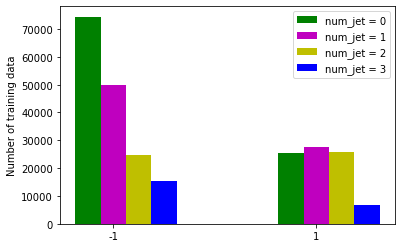
\includegraphics[scale=0.27]{labels_training.png}
    }
    \quad
    \subfloat[15th feature for 1$^{st}$ group \label{fig2}]{
        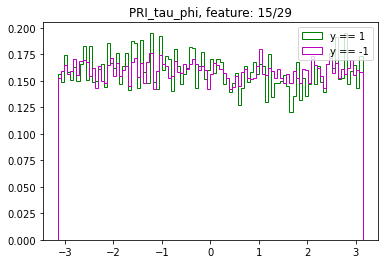
\includegraphics[scale=0.27]{feature_15_jet0.png}
    }
    \caption{Exploratory plots on the training dataset}
    \label{fig:empdistr}
\end{figure}

\subsection{Polynomial Feature Expansion}
This technique improves the representation power of linear models. For each feature, we add in the matrix its square, its square root and cubic root.
Moreover, we include all the pairwise products as new features.\\
\textcolor{red}{SCRIVERE SE LO RISOLVIAMO:} The optimal degree 2 of the polynomial expansion is found performing 4-fold cross-validation.

\subsection{Management of Outliers}
To deal with the presence of outliers, we fix $\alpha = 0.1$ and decide to cap the extreme values of each feature to the $\alpha$-quantile (for the lower tail) and to the 1-$alpha$-quantile (for the upper tail).

\section{Models and Methods}
\label{models}
After the pre-processing on the dataset, we implement several models to solve the classification task, which employ linear models and logistic regression.
Note that, as stated in \ref{categorical}, we use only the train data with a specific \emph{PRI\_jet\_num} to predict the label of test data belonging to the same group. \\
The methods considered are:
\begin{itemize}
    \item \textbf{Gradient Descent}
    \item \textbf{Stochastic Gradient Descent}, 
    \item \textbf{Least Squares} with Normal Equations
    \item \textbf{Logistic Regression}
    \end{itemize}
We implement the regularized versions as well, in order to reduce overfitting:
\begin{itemize}
\item \textbf{Lasso Regression}
\item \textbf{Ridge Regression}
\item \textbf{Regularized Logistic Regression}
\end{itemize}

The optimal hyper-parameter $\lambda$ is chosen with a 4-fold cross-validation. In Figure~\ref{fig:cross}, we report the accuracy trends for training and test set, which lead to our choice of hyper-parameters. \textcolor{red}{SCRIVERE MEGLIO QUANDO LO AVREMO}.
\\
\newline
\textcolor{red}{INSERIRE IMMAGINI DELLA CROSS-VALIDATION DI LAMBDA E DEGREE}
\\
\textcolor{red}{METODO FISTA}
\\
We implement also the K-nearest classification algorithm, which provides an accuracy of \textcolor{red}{INSERIRE}; this result is worse than the ones presented in Table~\ref{table1}, and the reason of this lies in the fact that the dimension of our dataset is extremely high, so the notion of distance does not make sense and the performance results also very computationally demanding.
\section{Results}
\label{results}
We report the accuracy results obtained for each method, with the optimal choice of hyper-parameters: \\

\textcolor{red}{INSERIRE I DATI GIUSTI}
\begin{center}
\label{table1}
\begin{tabular}{|c c c|} 
 \hline
 Method & Train Accuracy & Test Accuracy  \\ [0.5ex] 
 \hline\hline
 Least Squares GD & 6 & 87837  \\ 
 \hline
 Least Squares SGD & 7 & 78 \\
 \hline
 Least Squares Normal Eqs. & 545 & 778  \\
 \hline
 Lasso Regression & 545 & 18744  \\
 \hline
 Ridge Regression & 88 & 788  \\ 
 \hline
 Logistic Regression & 545 & 18744  \\
 \hline
 Reg. Logistic Regression & 545 & 18744  \\
 \hline
\end{tabular}
\end{center}



\section{Conclusion}

The best performance, with an accuracy on the test set of \textcolor{red}{INSERIRE NUMERO E POSIZIONE IN CLASSIFICA SE ALTA}, is obtained with the Lasso Regression; this highlights how even standard models can be powerful in solving complex classification tasks, and how regularization can help to reduce overfitting.
In addiction, we want to remark that a relevant part of the success of the task is up to the data preprocessing and interpretation.


\end{document}

